\part{Vers une synergie homme-machine}
    Alors que l'intelligence artificelle a un penchant "buzzword" utilisé par des entreprises pour 
    mieux vendre leur produit en faisant l'association IA égal à plus de performances, et que les 
    site et média d'informations montre du doigt l'intelligence artificelle comme le futur destructeur 
    d'emploi, il est important de souligner que les êtres humains sont passé par de telles phases 
    auparavant: \newline 

    \begin{itemize}
        \item La révolution agricole:En Europe, pendant le 18ième siècle moins de terres en jachère,
        << En 1840, 7 millions d'hectares c'est-à-dire 25\% 
        des terres européennes sont en jachère ; en 1900, il n'y a plus que 3
         millions d'hectares en jachère, c'est-à-dire 10 \% des terres. >>
         \footnote{source: \url{https://www.philisto.fr/cours-49-transformations-economiques-de-l-europe-xixe-siecle.html}}
         l'apparition de la moissonneuse et la batteuse à vapeur changent les méthodes agricoles 
         vers une agriculture orienté capitalisme. 
         Cette transformation a été globalement avantageuse pour tout le peuple, l'utilisation 
         des machines étant rare à cause de leur prix, l'utilisation d'animaux de traits ne 
         disparaitra que très progressivement ne laissant pas sans capacité de travail les personnes
         qui dépendaient de leur utilisation dans l'agriculture (la mecanisation ne s'effectuera 
         massivement qu'a partir de la fin de la seconde guerre mondiale). \newline 

         \item La révolution industrielle: c'est la transformation qui aura eu le plus grand impact,
         elle est decomposé en deux temp qui peuvent globalement être associé avec 
         l'utilisation de la machine à vapeur puis l'apparition de l'electricité, du gaz ainsi que 
         moteur à explosion, l'exode rural qui s'ensuit (fuir la campagne et son agriculture pour 
         rejoindre la ville et ses usines) et dû à une jeunesse formé à l'agriculture 
         qui ne voyait pas de futur dans l'agriculture et une opportunité dans l'industrie. \newline
    \end{itemize}

    cette période montre que l'homme et les nations ont les capacités pour s'adapter 
    aux paysages économiques en perpétuels changement, mais les challenges à surmonter 
    avec l'intelligence artificelle sont différents puisqu'elle va et a déjà bousculée tout 
    les domaines y compris l'agriculture et l'industrie, pour que cette 
    révolution soit aussi disruptives il y a de nombreux challenges à dépasser:
    \newline

    \begin{itemize}
        \item La resistance au changement.
        \item Problèmes inhérent à la technologie (traités plus loin).
        \item Le manque de confiance en l'intelligence artificelle. \newline
    \end{itemize}

    Les institutions ont aussi un jeu très important à jouer avec la mise en place 
    de taxe, lois et règlementations du domaine de l'intelligence artificelle.

    \chapter{Surmonter les problèmes inhérent au machine learning }
        Des problèmes empecheront l'intelligence artificelle notamment à cause de l'utilisation 
        du machine learning, technologie qui va rester d'actualité pendant de nombreuses années car nous
        avons qu'effleuré la surface et les possibilités de celle-ci.
        Tout d'abord le principe d'explicabilité, la difficulté de reproductibilité et enfin l'applicabilité 
        métiers sont les trois principaux points bloquants pour une évolution positive de 
        l'intelligence artificielle. \newline

        \section{Explicabilité et Interprétabilité}
            \subsection*{Définitions}
            Explicabilité: 
            \begin{quote}
                << Une décision algorithmique est dite explicable s’il est possible d’en rendre compte 
                explicitement à partir de données et caractéristiques connues de la situation. 
                Autrement dit, s’il est possible de mettre en relation les valeurs prises 
                par certaines variables (les caractéristiques) et leurs conséquences  
                sur la prévision, par exemple d’un score, et ainsi sur la décision. >>
                \footnote{Source: \url{https://perso.math.univ-toulouse.fr/mllaw/home/statisticien/explicabilite-des-decisions-algorithmiques/}}
                \newline 
            \end{quote}

            Interprétabilité:
            \begin{quote}
                << Une décision algorithmique est dite interprétable s’il est possible d’identifier 
                les caractéristiques ou variables qui participent le plus à la décision, 
                voire même d’en quantifier l’importance. >>
                \footnote{Source:\url{https://perso.math.univ-toulouse.fr/mllaw/home/statisticien/explicabilite-des-decisions-algorithmiques/}}
                \newline
            \end{quote}

            Une des raison de la resistance au changement est l'incapacité à comprendre 
            le fonctionnement interne d'une intelligence artificelle utilisant le machine learning, 
            ce qui rend une entreprise dépendant de cette dernière avec un maîtrise relative
            entre les mains des data scientists. \newline

            Prenon l'exemple d'un algorithme standard, par exemple un arbre syntaxique abstrait
            dans compilateur, il est aisé de comprendre le fonctionnement de chaque partie 
            de l'arbre et l'impact dans le cas du changement de la valeur d'un noeud.
            Dans le cas d'un algorithme de reconnaissance d'image par machine learning 
            il est bien plus difficile de comprendre les variables en jeux lors du changement 
            d'un pixel par exemple, aujourd'hui l'explicabilité et l'interprétabilité
            du deep learning est nulle. \newline

            \begin{figure}[H]
                \centering
                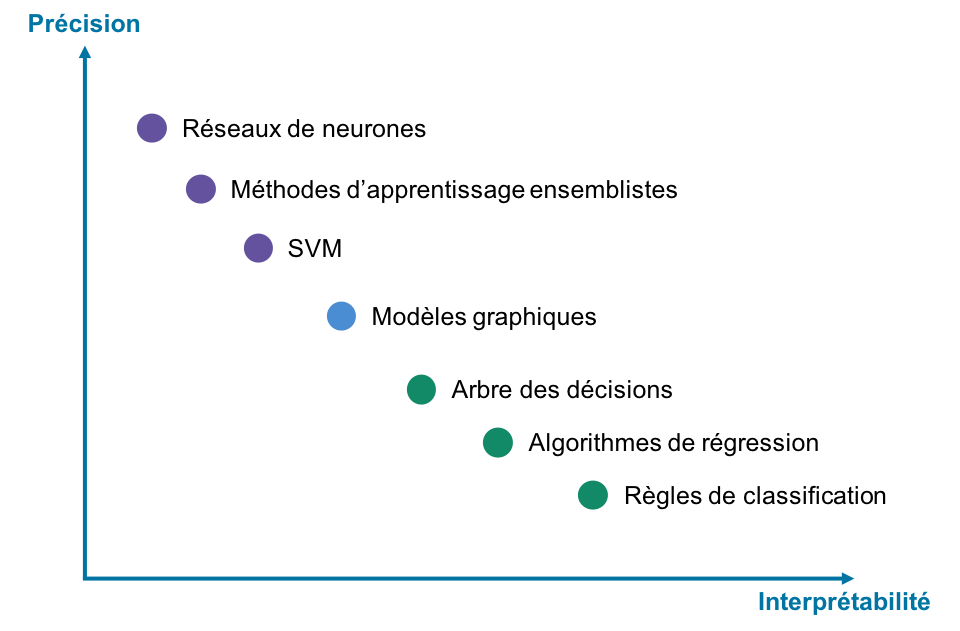
\includegraphics[width=0.7\textwidth]{Images/accvsint}
                \caption{Précision vs Interprétabilité - actuia.com}
                \label{fig:explicability}
            \end{figure}

            En réalité plus un algorithme de machine learning est précis et fiable 
            plus sont interprétabilité devient faible, le système <<deviens une boite 
            noire>>, malheureusement par défaut les réseaux de neurones semblent 
            être dans le bas du panier. \newline 
            
            Une intelligence artificelle en capacité de répondre aux besoins d'explicabilité 
            doit pouvoir répondre aux questions suivantes: \newline 

            \begin{itemize}
                \item Objectif d'une opération: pourquoi avoir fait cette action, 
                dans quel but ? \newline 
                \item Critères de choix d'une action: quelles ont été les critères 
                qui ont permis de séléctionner une action donnée par rapport aux 
                autres ? \newline
                \item Variables prises en compte: quelles variables ont été utilisées
                pour l'action ? \newline 
            \end{itemize}

            Sans ces réponse il est impossible de comprendre ce qui ce passe à "l'intérieur"
            de l'algorithme de machine learning qui deviens donc une "boite noire"
            cela réduit considérablement la confiance d'une entreprise dans le système,
            il faut en plus prendre en compte la difficulté à modifier un modèle correctement à 
            partir des résultats, ce qui augmente considérablement le temp d'optimisation.
            \newline

            Aujourd'hui avec le Règlement Européen sur la Protection des Données ou RGPD par son 
            acronyme, l'interprétabilité deviens un devoir des entrprises, comment 
            peut-on fournir à un client les choix qui ont permis d'accorder un crédit
            si l'intelligence artificelle qui fait ce choix est une boîte noire ?
            
            \begin{figure}[H]
                \centering
                
\includegraphics[width=0.7\textwidth]{Images/explicabilite}
                \caption{Enjeux de l'explicabilité - actuia.com}
                \label{fig:explicability}
            \end{figure}

            l'interprétabilité n'est pas forcément obligatoire pour tout les systèmes 
            faisant usage du machine learning, des systèmes basiques par exemple 
            mais dans quel cas l'interprétabilité est nécéssaire ?  \newline
    
            \begin{quote}
                << We argue that the need for interpretability
                stems from an incompleteness in the problem formalization, creating a fundamental barrier to
                optimization and evaluation. Note that incompleteness is distinct from uncertainty: the fused
                estimate of a missile location may be uncertain, but such uncertainty can be rigorously quantified
                and formally reasoned about. >>
                \footnote{source: Towards A Rigorous Science of Interpretable Machine Learning \newline
                Doshi-Velez and Been Kim \newline
                \url{https://arxiv.org/pdf/1702.08608.pdf}}
                \newline
            \end{quote}

        \newpage
        \section{Reproductibilité}
        L'explicabilité permettrait de faciliter la reproductibilité, tandis que sans celle-ci 
        aujourd'hui les data scientists rencontre une difficulté majeure: 
        l'incapacité à reproduire les modèles de machine learning d'autres data scientists 
        et chercheur voir même l'incapacité à reproduire ses propres modèles. \newline 
        
        La reproductibilité est essentielle pour assurer la pérénité d'un modèles de représentation, 
        et c'est la difficulté majeure car comment avoir un système fiable s'il est impossible 
        d'avoir les même résultats entre un environement de développement, de test et celui 
        utilisé en production ? l'interprétabilité permet de comprendre le fonctionnement 
        d'un modèle mais aussi d'en assurer le bon fonctionnement ce qui n'est pas le cas 
        pour une "boite noire" ou même si l'on obtiens des résultat semblable avec des données 
        identique il reste impossible de verifier la constance du cas de test en production. 
        \newline





        \section{Applicatibilité Métier}
            Cette problématique concerne l'identification des besoins auquels l'intelligence artificelle 
            peut répondre, comme indiqué dans la partie précèdente une des principales difficulté réside 
            dans l'application concrète de celle-ci, à quel(s) besoin(s) peut répondre une 
            intelligence artificelle qu'un algorithme "traditionnel" ne peut pas ? 
            \newline 

            L'utilité première du machine learning est de traiter rapidement une grande 
            quantité d'information plus ou moins impure avec éfficacité, la contrainte 
            réside dans la quantité d'informations qu'il faut pour réaliser un modèle 
            éfficace, si le domaine métier ne permet pas d'avoir des données en quantité 
            suffisante le machine learning est une technologie peu pertinente. 
            \newline 

            Les performances ou le non determinisme que permet l'intelligence artificelle
            peut ne pas être primordial, l'utilisation de cette technologie serait 
            aurait même un impact négatif avec au final de "l'over-engineering" 
            qui signifie l'utilisation d'une solution bien trop complexe et 
            difficile à maintenir pour résoudre un problème. 
            \newline  


    \chapter{Automatiser les taches sans grande valeur ajoutée}

        Nous avons vous dans la partie précédente que l'intelligence artificelle
        ne pourra pas remplacer l'intelligence artificelle dans tout 
        les domaines qui demande de la créativité, de l'empathie et globalement 
        la majorité des domaines qui demande des intéractions complexes entre 
        individus tel que la gestion de projet, l'analyse du besoin et la 
        diplomatie. Il faut donc étudier quels métiers peuvent être automatisés dans le futur proche,
        voici une classification des caractéristiques d'un métier qui peut être automatisé:
        \newline
        \begin{itemize}
            \item Taches simples et répétitives, répétition basique mais non absolue, des automates 
            comme dans les industrie automobiles peuvent remplir le rôle, on parle ici de tâche 
            répétitive mais non deterministes.
            \newline

            \item Communication simple avec un être humain tel que le démarchage téléphonique,
            gestion de demande administrative (statut d'un dossier, demande de document), 
            la reception / accueil où la gestion d'appel et d'agenda peut facilement être automatisé,
            le domaine comptable dans lequel il y a dèjà des offres qui automatise fortement 
            la comptabilité tel que QuickBooks et FreshBooks.
            \newline

            \item Taches simples non répétitives comme 
            les voitures taxi, les véhicules de livraison, l'objectif est d'aller d'un point A à 
            un point B. \newline
        \end{itemize}

        Il est important de souligner le fait que la possiblité d'automatisation d'un métiers 
        n'est pas une notion absolue, toutes les entreprises n'ont pas 
        les capacités financières pour investir dans l'intelligence artificelle, les petites entreprises 
        se recentreront sur la relation client humain à humains avec des services personnalisés,
        une autre possibilités et la complémentarité de l'usage d'IA qui conduit à une augmentation 
        du profit on peut cité par exemple des conseiller en investissement qui sont remplacés 
        par des intelligences artificelles en dehors des horaires standard. \newline

        La personnalisation des services est la partie bloquante de certains métiers 
        automatisable par IA, par exemple dans le domaine du secrétériat téléphonique,
        la valeur ajouté des centres d'appel est la personnalisation au plus près 
        des besoins du client de la gestion d'un appel, la diversité conséquente 
        des type d'appels et des personnalisations associés rendent l'utilisation 
        d'une intelligence artificelle très difficile, de plus l'argument financier 
        n'est pas en sa faveur puisque de lourd investissement en recherche et developpement
        seraient nécéssaire avec une répercution néfaste sur les prix pour les clients finaux 
        pour une impact faible sur la qualité, ceci est un exemple phare 
        d'un métier pouvant être automatisé mais dont les subtilités l'en empeche et 
        en font même la force.

        Plusieurs métiers ont déjà été automatisé non pas par une IA mais par des systèmes 
        autonomes, nous pouvons voir une tendance qui n'est pas à la destruction 
        d'emploi mais parfois même du contraire avec transformation de celui-ci\newline

        
        \section{Re-spécialisiation des métiers automatisés: le cas du caissier
        de banque et des distributeurs automatiques}
        
        L'apparition du premier guichet automatique banquaire en francee en 1968 
        aurait dù sonner le glas des caissier banquaire, aujourd'hui 
        plus communément connu sous le nom de conseiller ce qui donne un indice 
        sur l'évolution de leur métiers changé par une technologie disruptive.
        l'effet de l'arrivée des GAB a actuellement permis d'augmenter le 
        nombre d'agences de proximité avec l'augmentation de revenu de ces derniers.
        \newline

        Exemple aux États-Unis avec le graphe ci-dessus, avec une situation semblable en France 
        Le nombre de caissiers de banque a augmenté constament de manière 
        logarithmique depuis le debut des années 1970, l'explication est 
        le requalification du métier, aujourd'hui le conseiller 
        est plus orienté vers la relation client et endosse aussi le rôle 
        de commercial pour vendre des services de la banque à ses clients.


        \begin{figure}[H]
            \centering
            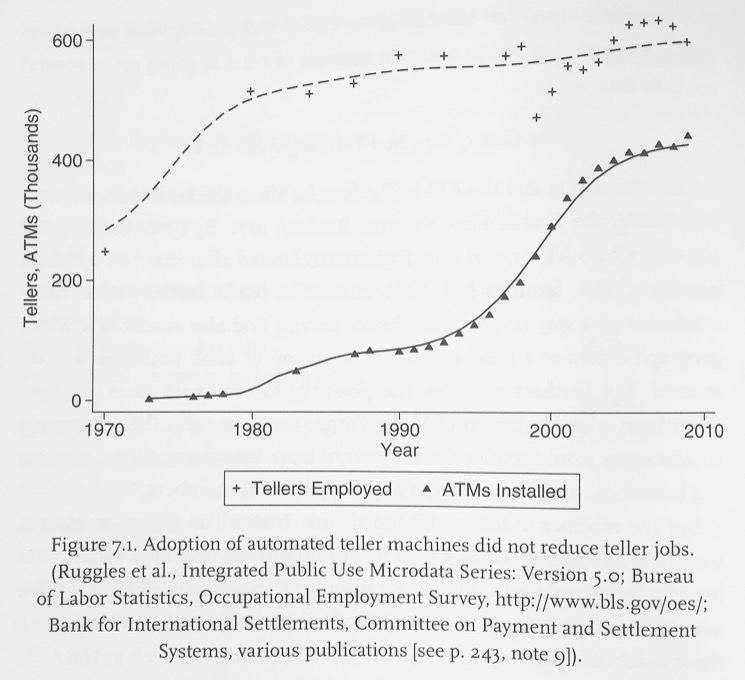
\includegraphics[width=0.9\textwidth]{Images/bankteller}
            \caption{Évolution des caissiers de banque et des distributeurs automatiques - 
            Bureau of labor statistics, Occupational Employement Survey }
            \label{fig:banktellerevolution}
        \end{figure}

        %as automation frees our time it increases the scope of what is possible we invent new ideas
        %new products
        %O-ring principle
        %automation: create more wealth in less time
        %build society with opportunity, problems is the institution
        % 

    \chapter{l'intelligence artificelle à notre service}
    \section{Le supermarché du futur}
    Le supermarché du futur est hautement connecté pour faciliter le plus possible 
    à la fois l'experience des clients et la réalisation des tâches pour 
    les employés. 

    Les caddies sont connecté pour traiter les données de déplacement qui seront 
    ensuite utilisée pour améliorer la disposition des rayons au sein du supermarché.

    le supermarché fonctionne autour d'un système sans caisse basé sur des caméra 
    et comme pour les supermarchés Amazon Go 
    \footnote{Amazon opens a supermarket with no checkouts:  \url{https://www.bbc.com/news/business-42769096}} 
    \newline

    Gestion de rayon assisté par intelligence artificelle: 
    
    \begin{figure}[H]
        \centering
        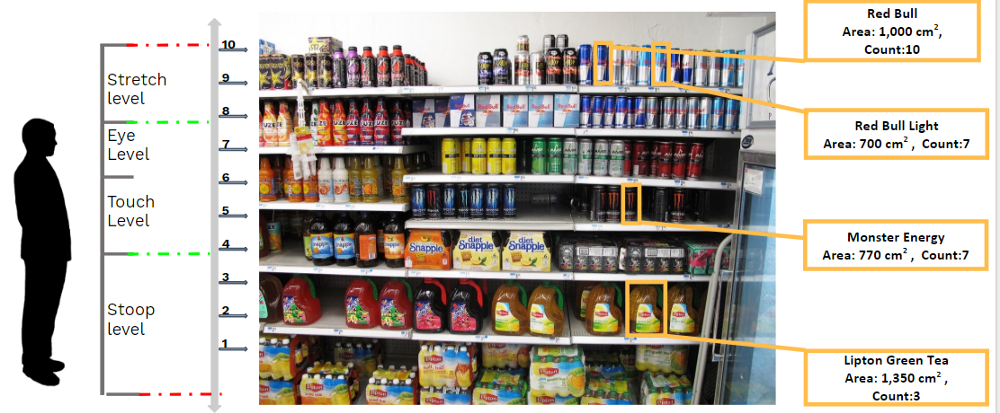
\includegraphics[width=1\textwidth]{Images/shelfAI}
        \caption{Gestion de rayon par IA - hackernoon.com }
        \label{fig:shelfAI}
    \end{figure}

    Gestion du placement en rayon en fonction des données d'achat et du déplacement 
    des caddies, inventaire automatique pour permettre de réduire 
    le gaspillage et éviter tout manque d'articles. \newline 

    Le système se base sur différent niveau de positionnement ainsi que les 
    zones les plus propices pour pousser à l'achat, par exemple 
    positionner les produit les plus acheté au "Touch Level" pour permettre 
    à un individu de prendre le produit rapidement, tandis qu'il faut mettre 
    les nouveaux produits ou produit à fort potentiel d'achat au niveau 
    des yeux pour inciter à l'achat. \newline 

    les employés au même titre que les caissier de banque lors de l'apparition
    des guichets automatiques bancaire, vont voir leur tâches redéfinie 
    et vont se reconcentrer sur l'accueil et le conseil client, avec 
    par exemple des rayons hautement spécialisés tandis que les denrées
    alimentaires "standards" sont livrés par drones ou directement via 
    des "drive", l'objectif étant de spécialiser les grandes surface 
    comme de grand magasins spécialisés. \newline 

    \section{Villes Intelligente}
    La gestion du traffic n'a pas changé depuis les année 60 
    et l'apparition des feu de traffic géré par ordinateur, avec 
    les avancement en terme de reconnaissance d'image et de machine learning 
    il serait possible d'implémenter la gestion du traffic par intelligence 
    artificielle pour optimiser au maximum le flot de circulation 
    mais aussi une réduction de la dégradation de l'asphalte en réduisant le 
    nombre d'arrêt, suppression des feu rouge inutile ce qui diminuerais 
    la congestion et par association la pollution et les temps de trajet. \newline
    
    Exemple: Surtrac ou Scalable Urban Traffic Control system

    \begin{figure}[H]
        \centering
        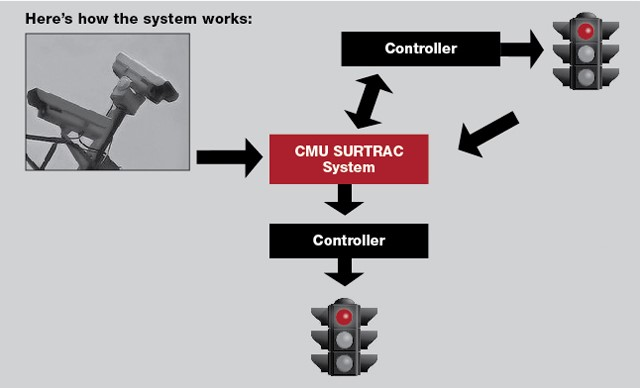
\includegraphics[width=0.9\textwidth]{Images/traffic}
        \caption{Gestion de traffic - makeasmartcity.com }
        \label{fig:trafficAI}
    \end{figure}
    
    1. les conditions actuelles du traffic sont extraites 
    depuis le flux vidéos de caméra 

    2. le système planifie le traffic et envoie les commandes au controlleur 

    3. la planification est envoyé à tout les controlleurs 

    4. ce cycle est répété au bout de quelques secondes 